\section{Algorithm}
\textbf{Vision Transformer (ViT)} is a new structure that first successfully adapted the Transformer Model from natural language processing applications for visual tasks. This structure is described in the paper published by Dosovitskiy et al. \cite{df01} in 2020 and quickly became a major trend in the deep learning world when working with images. The main difference between traditional computer vision approaches, which include convolutional neural networks (CNNs), is that ViT does not have any convolutional layers, using only attention arrays instead.

\subsection{Architecture}
\begin{figure}[h!]
  \centering
  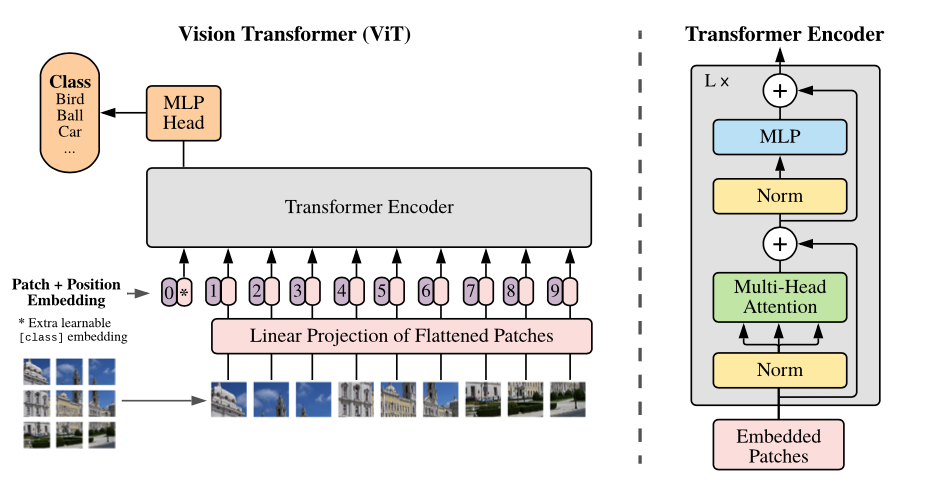
\includegraphics[width=1\textwidth]{images/vit_figure.png}
  \caption{ViT Architecture}\cite{df01}
  \label{fig:vit_architecture}
\end{figure}
The Vision Transformer (\textbf{ViT}), as illustrated in the Fig \ref{fig:vit_architecture} is designed to operate similarly to transformers used in natural language processing, but instead of processing words, it processes image patches. Below is a detailed breakdown of the architecture based on the diagram:
\subsection{Patch and Position Embedding}
\subsubsection{Input}: The Vision Transformer takes as input an image, which is a full rectangular surface and is first cut into square patches without overlap. Each patch is usually of dimension 16×16 pixels but may vary from this size in a given implementation.
\subsubsection{Flattening}: Each of these patches is then flattened into a vector. For example, for a patch of size $\mathbf{16}\times\mathbf{16}$ in RGB coloration, this equates to a vector of size $\mathbf{16}\times\mathbf{16} \times\mathbf{3}=768$.
\subsubsection{Patch Embedding}: The flat patches are mapped to a fixed-length vector using a linear projection that can be learned. This process is quite similar to how we have token embeddings in NLP.
\subsubsection{Positional Embedding}: Since transformers do not understand the position of patches with respect to others, it is necessary to append some positional information to every patch embedding. These embeddings specify in which area of the image each of the patches is situated.
This step concludes with a sequence of embedded patches that consists of the patch content in addition to its respective geographical location.
\subsection{Transformer Encoder}
\subsubsection{Input Sequence}: Following the patch embedding and the position encoding, the input transforms into a series of vectors (or tokens), each of the token being a patch in the respective position in the image.
\subsubsection{Class Token}: The architecture incorporates a class token that is learnable at the start of the sequence, much in the same way left a “class” token in NLP transformers known as “[CLS]” which gathers up information of all the patches and is ultimately used for classification.
\subsubsection{Transformer Layers}
The sequence of patch embeddings is joined with the class token and they are then transformed through a series of Transformer Encoder layers. Each layer is made up of:
\begin{itemize}
    \item \textbf{Multi-Head Self-Attention:} The self-attention mechanism permits the model to make connections between various patches, hence it is able to comprehend the large image patches with the help of long-range dependencies.
    \item \textbf{Layer Normalization:} Normalization layers are used to maintain the training process volatile.
    \item \textbf{Feed-Forward Neural Network (MLP):} After the self-attention mechanism, a feed-forward neural network is applied to each token. This is typically a two-layer MLP with a ReLU activation function in between.
    \item \textbf{Residual Connections:} Residual connections are included in both the self-attention layer and the feed-forward neural network to make sure that the gradients flow smoothly during training.
\end{itemize}
This process is repeated for L layers, where L is the number of transformer encoder layers in the model.
\subsection{MLP Head for Classification}
\begin{itemize}
    \item At the end of the transformer encoder layers, the original sequence of patch tokens and also the class token is used for classification by the class token.
    \item The class token's output is fed into an MLP Head composed of one or more fully connected layers shrinking the capacity and a softmax or another activation function is then used for classification.
    \item \textbf{Output}: The output of this MLP head is the class label (e.g., bird, ball, car), which tells what the image is.
\end{itemize}